\chapter{Obilazak grafa}

Ovo poglavlje obrađuje dva temeljna
algoritma na grafovima:
pretraživanje u dubinu i pretraživanje u širinu.
Oba algoritma dobivaju početni
čvor u grafu
i posjećuju sve čvorove do kojih se može doći
iz početnog čvora.
Razlika između algoritama je u redoslijedu
kojim posjećuju čvorove.

\section{Pretraživanje u dubinu}

\index{pretraživanje u dubinu}

\key{Pretraživanje u dubinu} (DFS)
jednostavna je tehnika obilaska grafa.
Algoritam počinje u početnom čvoru
i nastavlja do svih ostalih čvorova koji su
dostižni iz početnog čvora
koristeći bridove grafa.

Pretraživanje u dubinu uvijek slijedi jedan
put u grafu sve dok pronalazi
nove čvorove.
Nakon toga vraća se u prethodne
čvorove i počinje istraživati druge dijelove grafa.
Algoritam prati posjećene čvorove,
tako da svaki čvor obradi samo jednom.

\subsubsection*{Primjer}

Razmotrimo kako pretraživanje u dubinu obrađuje
sljedeći graf:
\begin{center}
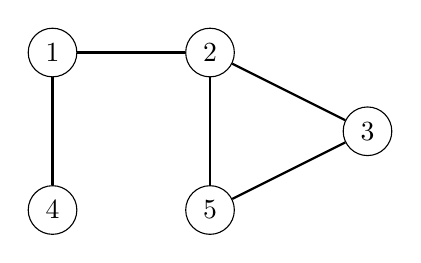
\begin{tikzpicture}
\node[draw, circle] (1) at (1,5) {$1$};
\node[draw, circle] (2) at (3,5) {$2$};
\node[draw, circle] (3) at (5,4) {$3$};
\node[draw, circle] (4) at (1,3) {$4$};
\node[draw, circle] (5) at (3,3) {$5$};

\path[draw,thick,-] (1) -- (2);
\path[draw,thick,-] (2) -- (3);
\path[draw,thick,-] (1) -- (4);
\path[draw,thick,-] (3) -- (5);
\path[draw,thick,-] (2) -- (5);
\end{tikzpicture}
\end{center}
Pretraživanje možemo započeti u bilo kojem čvoru grafa;
mi ćemo ga sada započeti u čvoru 1.

Pretraživanje najprije prelazi u čvor 2:
\begin{center}
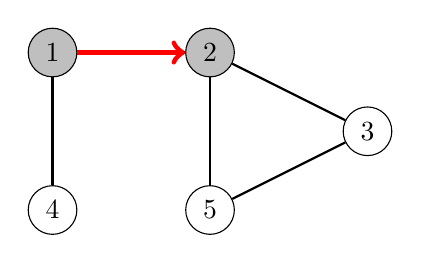
\begin{tikzpicture}
\node[draw, circle,fill=lightgray] (1) at (1,5) {$1$};
\node[draw, circle,fill=lightgray] (2) at (3,5) {$2$};
\node[draw, circle] (3) at (5,4) {$3$};
\node[draw, circle] (4) at (1,3) {$4$};
\node[draw, circle] (5) at (3,3) {$5$};

\path[draw,thick,-] (1) -- (2);
\path[draw,thick,-] (2) -- (3);
\path[draw,thick,-] (1) -- (4);
\path[draw,thick,-] (3) -- (5);
\path[draw,thick,-] (2) -- (5);

\path[draw=red,thick,->,line width=2pt] (1) -- (2);
\end{tikzpicture}
\end{center}
Nakon toga bit će posjećeni čvorovi 3 i 5:
\begin{center}
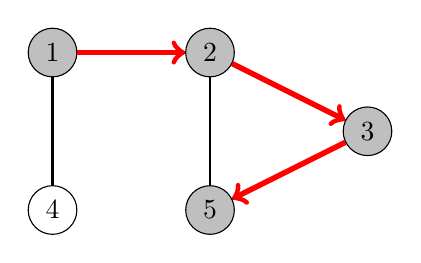
\begin{tikzpicture}
\node[draw, circle,fill=lightgray] (1) at (1,5) {$1$};
\node[draw, circle,fill=lightgray] (2) at (3,5) {$2$};
\node[draw, circle,fill=lightgray] (3) at (5,4) {$3$};
\node[draw, circle] (4) at (1,3) {$4$};
\node[draw, circle,fill=lightgray] (5) at (3,3) {$5$};

\path[draw,thick,-] (1) -- (2);
\path[draw,thick,-] (2) -- (3);
\path[draw,thick,-] (1) -- (4);
\path[draw,thick,-] (3) -- (5);
\path[draw,thick,-] (2) -- (5);

\path[draw=red,thick,->,line width=2pt] (1) -- (2);
\path[draw=red,thick,->,line width=2pt] (2) -- (3);
\path[draw=red,thick,->,line width=2pt] (3) -- (5);
\end{tikzpicture}
\end{center}
Susjedi čvora 5 su 2 i 3,
ali pretraživanje je oba već posjetilo,
pa je vrijeme za povratak u prethodne čvorove.
Također su i susjedi čvorova 3 i 2
već posjećeni, pa se sljedeće pomičemo
iz čvora 1 u čvor 4:
\begin{center}
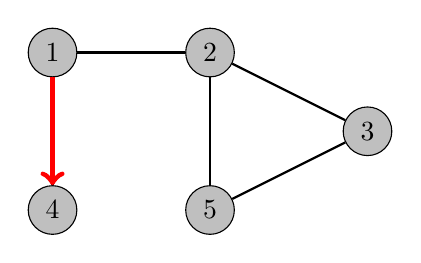
\begin{tikzpicture}
\node[draw, circle,fill=lightgray] (1) at (1,5) {$1$};
\node[draw, circle,fill=lightgray] (2) at (3,5) {$2$};
\node[draw, circle,fill=lightgray] (3) at (5,4) {$3$};
\node[draw, circle,fill=lightgray] (4) at (1,3) {$4$};
\node[draw, circle,fill=lightgray] (5) at (3,3) {$5$};

\path[draw,thick,-] (1) -- (2);
\path[draw,thick,-] (2) -- (3);
\path[draw,thick,-] (1) -- (4);
\path[draw,thick,-] (3) -- (5);
\path[draw,thick,-] (2) -- (5);

\path[draw=red,thick,->,line width=2pt] (1) -- (4);
\end{tikzpicture}
\end{center}
Nakon toga pretraživanje završava jer je posjetilo
sve čvorove.

Vremenska složenost pretraživanja u dubinu je $O(n+m)$,
gdje je $n$ broj čvorova, a $m$
broj bridova,
jer algoritam obrađuje svaki čvor i brid jednom.

\subsubsection*{Implementacija}

Pretraživanje u dubinu može se prikladno
implementirati pomoću rekurzije.
Sljedeća funkcija \texttt{dfs} započinje
pretraživanje u dubinu u zadanom čvoru.
Funkcija pretpostavlja da je graf
pohranjen kao liste susjedstva u nizu
\begin{lstlisting}
vector<int> adj[N];
\end{lstlisting}
te da se održava i niz
\begin{lstlisting}
bool visited[N];
\end{lstlisting}
koji prati posjećene čvorove.
Na početku je svaka vrijednost niza \texttt{false},
a kad pretraživanje dođe u čvor $s$,
vrijednost \texttt{visited}[$s$] postaje \texttt{true}.
Funkciju možemo implementirati ovako:
\begin{lstlisting}
void dfs(int s) {
    if (visited[s]) return;
    visited[s] = true;
    // obradi čvor s
    cout << s << " ";
    for (auto u: adj[s]) {
        dfs(u);
    }
}
\end{lstlisting}

\section{Pretraživanje u širinu}

\index{pretraživanje u širinu}

\key{Pretraživanje u širinu} (BFS) posjećuje čvorove
u rastućem redoslijedu njihove udaljenosti
od početnog čvora.
Stoga pomoću pretraživanja u širinu možemo izračunati
udaljenost od početnog čvora do svih
ostalih čvorova.
Međutim, pretraživanje u širinu teže je
implementirati od pretraživanja u dubinu.

Pretraživanje u širinu prolazi kroz čvorove
razinu po razinu.
Najprije pretraživanje istražuje čvorove čija je
udaljenost od početnog čvora 1,
zatim čvorove čija je udaljenost 2 i tako dalje.
Taj se postupak nastavlja dok svi čvorovi
ne budu posjećeni.

\subsubsection*{Primjer}

Razmotrimo kako pretraživanje u širinu obrađuje
sljedeći graf:

\begin{center}
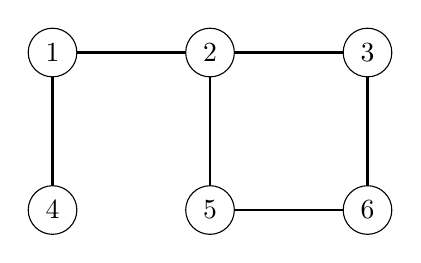
\begin{tikzpicture}
\node[draw, circle] (1) at (1,5) {$1$};
\node[draw, circle] (2) at (3,5) {$2$};
\node[draw, circle] (3) at (5,5) {$3$};
\node[draw, circle] (4) at (1,3) {$4$};
\node[draw, circle] (5) at (3,3) {$5$};
\node[draw, circle] (6) at (5,3) {$6$};

\path[draw,thick,-] (1) -- (2);
\path[draw,thick,-] (2) -- (3);
\path[draw,thick,-] (1) -- (4);
\path[draw,thick,-] (3) -- (6);
\path[draw,thick,-] (2) -- (5);
\path[draw,thick,-] (5) -- (6);
\end{tikzpicture}
\end{center}
Pretpostavimo da pretraživanje počinje u čvoru 1.
Najprije obrađujemo sve čvorove do kojih se može doći
iz čvora 1 pomoću jednog brida:
\begin{center}
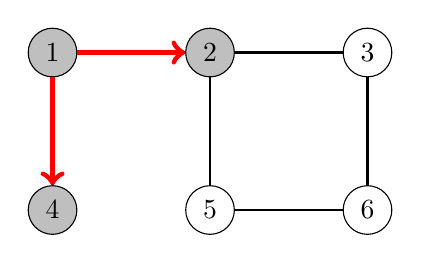
\begin{tikzpicture}
\node[draw, circle,fill=lightgray] (1) at (1,5) {$1$};
\node[draw, circle,fill=lightgray] (2) at (3,5) {$2$};
\node[draw, circle] (3) at (5,5) {$3$};
\node[draw, circle,fill=lightgray] (4) at (1,3) {$4$};
\node[draw, circle] (5) at (3,3) {$5$};
\node[draw, circle] (6) at (5,3) {$6$};

\path[draw,thick,-] (1) -- (2);
\path[draw,thick,-] (2) -- (3);
\path[draw,thick,-] (1) -- (4);
\path[draw,thick,-] (3) -- (6);
\path[draw,thick,-] (2) -- (5);
\path[draw,thick,-] (5) -- (6);

\path[draw,thick,-] (1) -- (2);
\path[draw,thick,-] (2) -- (3);
\path[draw,thick,-] (1) -- (4);
\path[draw,thick,-] (2) -- (5);

\path[draw=red,thick,->,line width=2pt] (1) -- (2);
\path[draw=red,thick,->,line width=2pt] (1) -- (4);
\end{tikzpicture}
\end{center}
Nakon toga prelazimo na čvorove 3 i 5:
\begin{center}
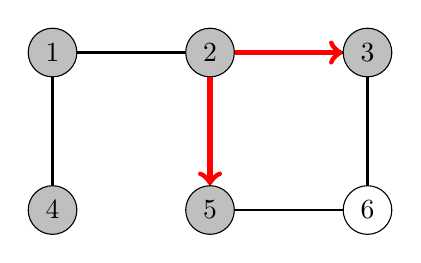
\begin{tikzpicture}
\node[draw, circle,fill=lightgray] (1) at (1,5) {$1$};
\node[draw, circle,fill=lightgray] (2) at (3,5) {$2$};
\node[draw, circle,fill=lightgray] (3) at (5,5) {$3$};
\node[draw, circle,fill=lightgray] (4) at (1,3) {$4$};
\node[draw, circle,fill=lightgray] (5) at (3,3) {$5$};
\node[draw, circle] (6) at (5,3) {$6$};

\path[draw,thick,-] (1) -- (2);
\path[draw,thick,-] (2) -- (3);
\path[draw,thick,-] (1) -- (4);
\path[draw,thick,-] (3) -- (6);
\path[draw,thick,-] (2) -- (5);
\path[draw,thick,-] (5) -- (6);

\path[draw,thick,-] (1) -- (2);
\path[draw,thick,-] (2) -- (3);
\path[draw,thick,-] (1) -- (4);
\path[draw,thick,-] (2) -- (5);

\path[draw=red,thick,->,line width=2pt] (2) -- (3);
\path[draw=red,thick,->,line width=2pt] (2) -- (5);
\end{tikzpicture}
\end{center}
Na kraju posjećujemo čvor 6:
\begin{center}
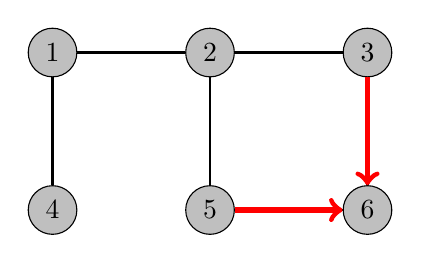
\begin{tikzpicture}
\node[draw, circle,fill=lightgray] (1) at (1,5) {$1$};
\node[draw, circle,fill=lightgray] (2) at (3,5) {$2$};
\node[draw, circle,fill=lightgray] (3) at (5,5) {$3$};
\node[draw, circle,fill=lightgray] (4) at (1,3) {$4$};
\node[draw, circle,fill=lightgray] (5) at (3,3) {$5$};
\node[draw, circle,fill=lightgray] (6) at (5,3) {$6$};

\path[draw,thick,-] (1) -- (2);
\path[draw,thick,-] (2) -- (3);
\path[draw,thick,-] (1) -- (4);
\path[draw,thick,-] (3) -- (6);
\path[draw,thick,-] (2) -- (5);
\path[draw,thick,-] (5) -- (6);

\path[draw,thick,-] (1) -- (2);
\path[draw,thick,-] (2) -- (3);
\path[draw,thick,-] (1) -- (4);
\path[draw,thick,-] (2) -- (5);

\path[draw=red,thick,->,line width=2pt] (3) -- (6);
\path[draw=red,thick,->,line width=2pt] (5) -- (6);
\end{tikzpicture}
\end{center}
Sada smo izračunali udaljenosti
od početnog čvora do svih čvorova grafa.
Udaljenosti su sljedeće:

\begin{tabular}{ll}
\\
čvor & udaljenost \\
\hline
1 & 0 \\
2 & 1 \\
3 & 2 \\
4 & 1 \\
5 & 2 \\
6 & 3 \\
\\
\end{tabular}

Kao i kod pretraživanja u dubinu,
vremenska složenost pretraživanja u širinu
je $O(n+m)$, gdje je $n$ broj čvorova,
a $m$ broj bridova.

\subsubsection*{Implementacija}

Pretraživanje u širinu teže je
implementirati od pretraživanja u dubinu,
jer algoritam posjećuje čvorove
u različitim dijelovima grafa.
Tipična implementacija temelji se na
redu koji sadrži čvorove.
U svakom koraku obrađuje se
sljedeći čvor u redu.

Sljedeći kod pretpostavlja da je graf pohranjen
kao liste susjedstva i održava sljedeće
strukture podataka:
\begin{lstlisting}
queue<int> q;
bool visited[N];
int distance[N];
\end{lstlisting}

Red \texttt{q}
sadrži čvorove koje treba obraditi
u rastućem redoslijedu njihove udaljenosti.
Novi čvorovi uvijek se dodaju na kraj
reda, a čvor na početku
reda sljedeći je čvor za obradu.
Niz \texttt{visited} pokazuje
koje je čvorove pretraživanje već posjetilo,
a niz \texttt{distance} sadržavat će
udaljenosti od početnog čvora do svih čvorova grafa.

Pretraživanje možemo implementirati ovako,
počevši u čvoru $x$:
\begin{lstlisting}
visited[x] = true;
distance[x] = 0;
q.push(x);
while (!q.empty()) {
    int s = q.front(); q.pop();
    // obradi čvor s
    cout << s << " ";
    for (auto u : adj[s]) {
        if (visited[u]) continue;
        visited[u] = true;
        distance[u] = distance[s]+1;
        q.push(u);
    }
}
\end{lstlisting}

\section{Primjene}

Pomoću algoritama za obilazak grafa
možemo provjeriti mnoga svojstva grafova.
Obično se mogu upotrijebiti i pretraživanje u dubinu
i pretraživanje u širinu,
ali je u praksi pretraživanje u dubinu
bolji izbor jer ga je
lakše implementirati.
U sljedećim primjenama
pretpostavljat ćemo da je graf neusmjeren.

\subsubsection{Provjera povezanosti}

\index{povezan graf}

Graf je povezan ako postoji put
između bilo koja dva čvora grafa.
Stoga možemo provjeriti je li graf povezan
tako da započnemo u proizvoljnom čvoru i
utvrdimo možemo li doći do svih ostalih čvorova.

Na primjer, u grafu
\begin{center}
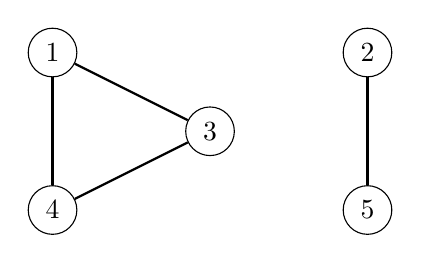
\begin{tikzpicture}
\node[draw, circle] (2) at (7,5) {$2$};
\node[draw, circle] (1) at (3,5) {$1$};
\node[draw, circle] (3) at (5,4) {$3$};
\node[draw, circle] (5) at (7,3) {$5$};
\node[draw, circle] (4) at (3,3) {$4$};

\path[draw,thick,-] (1) -- (3);
\path[draw,thick,-] (1) -- (4);
\path[draw,thick,-] (3) -- (4);
\path[draw,thick,-] (2) -- (5);
\end{tikzpicture}
\end{center}
pretraživanje u dubinu iz čvora $1$ posjećuje
sljedeće čvorove:
\begin{center}
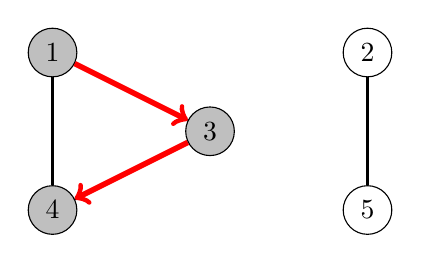
\begin{tikzpicture}
\node[draw, circle] (2) at (7,5) {$2$};
\node[draw, circle,fill=lightgray] (1) at (3,5) {$1$};
\node[draw, circle,fill=lightgray] (3) at (5,4) {$3$};
\node[draw, circle] (5) at (7,3) {$5$};
\node[draw, circle,fill=lightgray] (4) at (3,3) {$4$};

\path[draw,thick,-] (1) -- (3);
\path[draw,thick,-] (1) -- (4);
\path[draw,thick,-] (3) -- (4);
\path[draw,thick,-] (2) -- (5);

\path[draw=red,thick,->,line width=2pt] (1) -- (3);
\path[draw=red,thick,->,line width=2pt] (3) -- (4);

\end{tikzpicture}
\end{center}

Budući da pretraživanje nije posjetilo sve čvorove,
možemo zaključiti da graf nije povezan.
Na sličan način možemo pronaći i sve komponente povezanosti
grafa tako da prolazimo kroz čvorove i uvijek
pokrenemo novo pretraživanje u dubinu ako trenutni čvor
još ne pripada nijednoj komponenti.

\subsubsection{Pronalaženje ciklusa}

\index{ciklus}

Graf sadrži ciklus ako tijekom obilaska grafa
pronađemo čvor čiji je susjed (različit od
prethodnog čvora na trenutnom putu) već
posjećen.
Na primjer, graf
\begin{center}
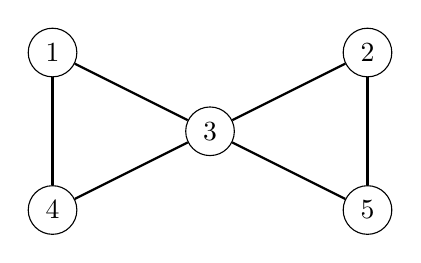
\begin{tikzpicture}
\node[draw, circle] (2) at (7,5) {$2$};
\node[draw, circle] (1) at (3,5) {$1$};
\node[draw, circle] (3) at (5,4) {$3$};
\node[draw, circle] (5) at (7,3) {$5$};
\node[draw, circle] (4) at (3,3) {$4$};

\path[draw,thick,-] (1) -- (3);
\path[draw,thick,-] (1) -- (4);
\path[draw,thick,-] (3) -- (4);
\path[draw,thick,-] (2) -- (5);
\path[draw,thick,-] (2) -- (3);
\path[draw,thick,-] (3) -- (5);
\end{tikzpicture}
\end{center}
sadrži dva ciklusa, a jedan od njih
možemo pronaći ovako:
\begin{center}
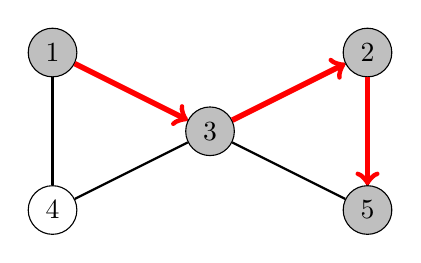
\begin{tikzpicture}
\node[draw, circle,fill=lightgray] (2) at (7,5) {$2$};
\node[draw, circle,fill=lightgray] (1) at (3,5) {$1$};
\node[draw, circle,fill=lightgray] (3) at (5,4) {$3$};
\node[draw, circle,fill=lightgray] (5) at (7,3) {$5$};
\node[draw, circle] (4) at (3,3) {$4$};

\path[draw,thick,-] (1) -- (3);
\path[draw,thick,-] (1) -- (4);
\path[draw,thick,-] (3) -- (4);
\path[draw,thick,-] (2) -- (5);
\path[draw,thick,-] (2) -- (3);
\path[draw,thick,-] (3) -- (5);

\path[draw=red,thick,->,line width=2pt] (1) -- (3);
\path[draw=red,thick,->,line width=2pt] (3) -- (2);
\path[draw=red,thick,->,line width=2pt] (2) -- (5);

\end{tikzpicture}
\end{center}
Nakon prelaska iz čvora 2 u čvor 5 primjećujemo da je
susjed 3 čvora 5 već posjećen.
Dakle, graf sadrži ciklus koji prolazi kroz čvor 3,
na primjer, $3 \rightarrow 2 \rightarrow 5 \rightarrow 3$.

Drugi način da utvrdimo sadrži li graf ciklus
jest da jednostavno izračunamo broj čvorova i bridova
u svakoj komponenti.
Ako komponenta sadrži $c$ čvorova i nema ciklusa,
mora sadržavati točno $c-1$ bridova
(pa mora biti stablo).
Ako ima $c$ ili više bridova, komponenta
sigurno sadrži ciklus.

\subsubsection{Provjera bipartitnosti}

\index{bipartitni graf}

Graf je bipartitan ako se njegovi čvorovi mogu obojiti
dvjema bojama tako da nema susjednih
čvorova iste boje.
Iznenađujuće je jednostavno provjeriti je li graf
bipartitan pomoću algoritama za obilazak grafa.

Ideja je obojiti početni čvor plavom bojom,
sve njegove susjede crvenom, sve njihove susjede plavom i tako dalje.
Ako u nekom trenutku pretraživanja primijetimo da
dva susjedna čvora imaju istu boju,
to znači da graf nije bipartitan.
Inače je graf bipartitan i pronašli smo
jedno bojenje.

Na primjer, graf
\begin{center}
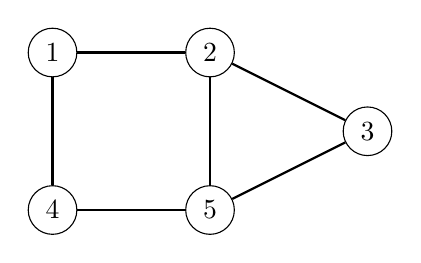
\begin{tikzpicture}
\node[draw, circle] (2) at (5,5) {$2$};
\node[draw, circle] (1) at (3,5) {$1$};
\node[draw, circle] (3) at (7,4) {$3$};
\node[draw, circle] (5) at (5,3) {$5$};
\node[draw, circle] (4) at (3,3) {$4$};

\path[draw,thick,-] (1) -- (2);
\path[draw,thick,-] (2) -- (5);
\path[draw,thick,-] (5) -- (4);
\path[draw,thick,-] (4) -- (1);
\path[draw,thick,-] (2) -- (3);
\path[draw,thick,-] (5) -- (3);
\end{tikzpicture}
\end{center}
nije bipartitan, jer pretraživanje iz čvora 1
teče ovako:
\begin{center}
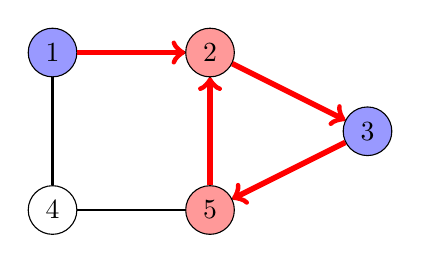
\begin{tikzpicture}
\node[draw, circle,fill=red!40] (2) at (5,5) {$2$};
\node[draw, circle,fill=blue!40] (1) at (3,5) {$1$};
\node[draw, circle,fill=blue!40] (3) at (7,4) {$3$};
\node[draw, circle,fill=red!40] (5) at (5,3) {$5$};
\node[draw, circle] (4) at (3,3) {$4$};

\path[draw,thick,-] (1) -- (2);
\path[draw,thick,-] (2) -- (5);
\path[draw,thick,-] (5) -- (4);
\path[draw,thick,-] (4) -- (1);
\path[draw,thick,-] (2) -- (3);
\path[draw,thick,-] (5) -- (3);

\path[draw=red,thick,->,line width=2pt] (1) -- (2);
\path[draw=red,thick,->,line width=2pt] (2) -- (3);
\path[draw=red,thick,->,line width=2pt] (3) -- (5);
\path[draw=red,thick,->,line width=2pt] (5) -- (2);
\end{tikzpicture}
\end{center}
Primjećujemo da su i čvor 2 i čvor 5
crvene boje, a susjedni su čvorovi u grafu.
Dakle, graf nije bipartitan.

Ovaj algoritam uvijek radi jer, kad
su na raspolaganju samo dvije boje,
boja početnog čvora u komponenti
određuje boje svih ostalih čvorova u toj komponenti.
Nije važno je li
početni čvor crven ili plav.

Primijetimo da je u općem slučaju
teško utvrditi mogu li se čvorovi
grafa obojiti pomoću $k$ boja
tako da nikoja dva susjedna čvora nemaju istu boju.
Čak i kad je $k=3$, nije poznat nijedan efikasan algoritam,
nego je zadatak NP-težak.
